%%% LaTeX Template
%%% This template can be used for both articles and reports.
%%%
%%% Copyright: http://www.howtotex.com/
%%% Date: February 2011

%%% Preamble
\documentclass[paper=a4, fontsize=11pt]{scrartcl}	% Article class of KOMA-script with 11pt font and a4 format


\usepackage[english]{babel}															% English language/hyphenation
\usepackage[protrusion=true,expansion=true]{microtype}				% Better typography
\usepackage{amsmath,amsfonts,amsthm}										% Math packages
\usepackage[pdftex]{graphicx}														% Enable pdflatex
%\usepackage{color,transparent}													% If you use color and/or transparency
\usepackage[hang, small,labelfont=bf,up,textfont=it,up]{caption}	% Custom captions under/above floats
\usepackage{epstopdf}																	% Converts .eps to .pdf
\usepackage{subfig}																		% Subfigures
\usepackage{booktabs}																	% Nicer tables
\usepackage{hyperref}


\usepackage{tikz}

\usepackage{graphicx}
\usetikzlibrary{shapes.geometric, arrows}

%%% Advanced verbatim environment
\usepackage{verbatim}
\usepackage{fancyvrb}
\DefineShortVerb{\|}								% delimiter to display inline verbatim text


%%% Custom sectioning (sectsty package)
\usepackage{sectsty}								% Custom sectioning (see below)
\allsectionsfont{%									% Change font of al section commands
	\usefont{OT1}{bch}{b}{n}%					% bch-b-n: CharterBT-Bold font
%	\hspace{15pt}%									% Uncomment for indentation
	}

\sectionfont{%										% Change font of \section command
	\usefont{OT1}{bch}{b}{n}%					% bch-b-n: CharterBT-Bold font
	\sectionrule{0pt}{0pt}{-5pt}{0.8pt}%	% Horizontal rule below section
	}


%%% Custom headers/footers (fancyhdr package)
\usepackage{fancyhdr}
\pagestyle{fancyplain}
\fancyhead{}														% No page header
\fancyfoot[C]{\thepage}										% Pagenumbering at center of footer

\renewcommand{\headrulewidth}{0pt}				% Remove header underlines
\renewcommand{\footrulewidth}{0pt}				% Remove footer underlines
\setlength{\headheight}{13.6pt}

%%% Equation and float numbering
\numberwithin{equation}{section}															% Equationnumbering: section.eq#
\numberwithin{figure}{section}																% Figurenumbering: section.fig#
\numberwithin{table}{section}																% Tablenumbering: section.tab#


%%% Title	
\title{ \vspace{-1in} 	\usefont{OT1}{bch}{b}{n}
		\huge \strut 3D ALGORITHM RECONSTRUCTION \strut \\
		\Large \bfseries \strut starting from a Point Cloud \strut
}

\date{}

%%% Begin document
\begin{document}
\maketitle
\section{INTRODUCTION}
After completing the  3D registration we pass to the next step that is the  3D reconstruction\\ 
One of the largest challenges in reconstructing surfaces robustly and accurately
is dealing with the many anomalies that are present in data that are obtained from
the scanning of real-world objects\\
Before to be able to reconstruct the 3D model we has faced some problems like the noise on the point cloud or high density of point.Inaccuracies in scanning devices createsq noisy data,and point sampling is often non-uniform.\\ Constructing a surface in the presence of these data anomalies is a difficult problem.In addition scanning technologies have driven a dramatic increase in the size of datasets available for reconstruction, with datasets now exceeding one billion point samples.As a result, space and time efficiency have become critical in the development of effective reconstruction algorithms surface reconstruction
\\
The reconstruction can be summarized like in scheme below:\\
\vspace{3pt}
\begin{center}
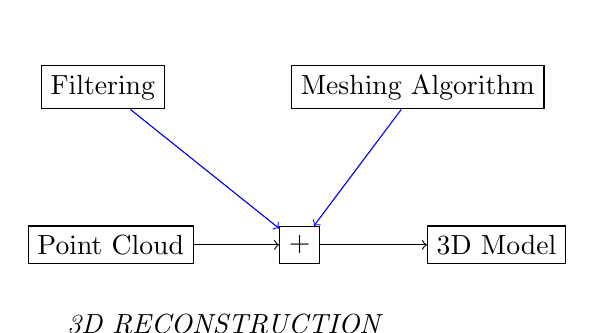
\begin{tikzpicture}
\node[draw] (ArgumentA) at (10.1,0) {Point Cloud};
\node[draw] (ArgumentB) at (15,0) {3D Model};
\node[draw] (ArgumentC) at (10,2) {Filtering};
\node[draw] (ArgumentD) at (14,2) {Meshing Algorithm};
\draw node[draw=black] (Joint) at (12.5,0) {+};

\draw[->] (ArgumentA) to (Joint);

\draw[->] (Joint) to (ArgumentB);
\draw[->,draw=blue] (ArgumentC) to (Joint);
\draw[->,draw=blue] (ArgumentD) to (Joint);

\node at (11.5, -1.0) {\textit{ 3D 	RECONSTRUCTION}};
\end{tikzpicture}
\end{center}
\vspace{3pt}
In our specific case the Point Cloud that we receive from the registration class was quite noisy, with a high density of point and we front even another problem "the extralayer of the surface" for better understand this problem we can see the following image:\\
 \begin{center}
 	
 	\includegraphics[width=45mm]{Noisy.jpg}
 	\includegraphics[width=40mm]{Noisy2.jpg}
 	
 \end{center}
The different techniques used for making 3D reconstruction will be discussed and tested from different aspects.This is done in order to find the most optimal reconstruction technique.
 
 
 


 

\section{ PREPARING THE CLOUD}
Before going into the implementation of the algorithms : greedy triangulation, marching cube and Poisson,it is necessary to look at the input data that is provided to these algorithms and how it is processed, so before give the point cloud tho this algorithm we have to do some operation on the point cloud:
\subsection{filtering}
Because the received point cloud it was oversampled first of all we decide to elaborate on it some filtering operation: 
\begin{itemize}
	\item PassThrough this filter iterates through the entire input Point Cloud,and  automatically filtering the non-finite points and the points outside to one presetted interval specified
	\item The VoxelGrid class creates a 3D voxel grid, as a set of tiny 3D boxes in space, over the input point cloud data. Then, in each voxel all the points present will be approximated with their centroid. This approach is a bit slower than approximating them with the center of the voxel, but it represents the underlying surface more accurately.
\end{itemize}
\subsection{MLS smoothing}
The first step taken after preparing the cloud is to smooth it using Moving Least Squares(MLS). As explained by [Alexa, Behr, Cohen-Or, Fleishman, Levin, and Silva, 2003] the idea behind MLS is to have a data set of points $P = \{pi\}$ that constructs a smooth surface SP , however, instead of using the original data set of points P, a reduced set $R = \{ri\}$ is created and a new surface SR is defined.

\begin{center}
    \includegraphics[width=50mm]{MLS.jpg}    
	\includegraphics[width=20mm]{ordinateMLS.jpg}

		


\end{center}

\begin{center}
	

	
	
	
\end{center}
The MLS smoothing is done before any reconstruction algorithm is applied. Another
smoothing method is also used, however only applied after the reconstruction is complete.
\subsection{Normalization}
In order to use the cloud properly for the reconstruction, a cloud with both x, y and z values and normal information is needed.
Many methods of surface reconstructions require normal associated with the point
clouds, the normal can either be oriented or unoriented. Normals that do not have a
direction are called unoriented normal, which means it is to be expected the normal to be pointing either on the inside or outside of the surface. This sort of information is useful to determine planar regions in a point cloud, projecting a point onto an approximated surface or achieving covariance matrix. An oriented normal on the other hand have consistent directions and it is known which point outside or inside of the surface.[Bergeret al.].\\
The problem of determining the normal to a point on the surface is approximated by the problem of estimating the normal of a plane tangent to the surface, which in turn becomes a least-square plane fitting estimation problem. The solution for estimating the surface normal is therefore reduced to an analysis of the eigenvectors and eigenvalues (or PCA – Principal Component Analysis) of a covariance matrix created from the nearest neighbours of the query point.\url{pointcloud.org}.\\

\section{MESHING ALGORITHMS}
At this point the point cloud is ready for the surface reconstruction.\\
As I mentioned before there are many algorithms for 3D reconstruction. In our work we compare the reconstruction of 3 of them. 

\subsection{Greedy Triangulation}
This is an iterative algorithm developed by "Zoltan Csaba Marton".
The focus of Fast Triangulation(FT) is to keep a list of possible points that can be connected to create a mesh.\\
FT is obtained by adding short compatible edges between points of the cloud, where these edges cannon cross previously formed edges between others point.
Fast Triangulation contains accurate and computationally efficient triangulations when the points are planar. However, a big difference can be noticed when the triangulations are non-planar.\\
The method works by maintaining a list of points from which the mesh can be grown and extending it until all possible points are connected. It can deal with unorganized points, coming from one or multiple scans, and having multiple connected parts. It works best if the surface is locally smooth and there are smooth transitions between areas with different point densities.\\
In the Point Cloud Library, fast triangulation works locally, however it allows the specification of the required features to be focused on. Such parameters are neighbourhood size of the search, the search radius and the angle between surfaces.
The surface created by this algorithm is not continuous and can contain holes, this was one of the reason that lead us to not use FT for reconstruct the meshes.\\
In the image below is illustrated the result obtained:
  \begin{center}
  	
  	\includegraphics[width=50mm]{triangulation.jpg}
  	
  \end{center}
\subsection{Poisson}
There are a multitude of surface reconstruction techniques, however each one of them
poses a number of difficulties when it is applied to data points.
But because watertight mesh was one of the prefixed setted point,at the end, we decided to use Poisson Algorithm Reconstruction. 
The Poisson reconstruction uses the Poisson equation, which is also known to
be used in systems that perform tone mapping, 
uid mechanics and mesh editing. The
Poisson reconstruction approached by Michael Kazhdan, Matthew Bolitho and Hugues
Hope has set as goal to reconstruct a watertight model.
It need in input the normal direction, respect to the surface, for each points of the cloud.\\
By its nature, this algorithm can only be used with watertight or closed object. This can be problematic when we get the points cloud  through Kinect, in fact the acquisition that we make not always respect this Property, as we can see in our model the head is not a close object.
In our specific case at the head and feet  can be noticed that the Poisson reconstruction connects the regions, which poses some limitations in the use of Poisson reconstruction, even more Poisson reconstruction has a high noisy sensitivity, we can see this in the images below:\\
\begin{center}
	
	\includegraphics[width=40mm]{reconstruction.jpg}\\
	
\end{center}



\subsection{Postprocessing algorithm Laplacian}
The obtained result was still a lot noisy, for having a better result in terms of surface problem we decide to apply a post smoothing method.\\
The smoothing method used is MeshSmoothingLaplacianVTK. This is a laplacian
smoothing method from the VTK library. As described in the documentation for
the original VTK smoothing method: \textit{"The effect is to "relax" the mesh, making the cells better shaped and the vertices more evenly distributed". [Visualization Toolkit}, 2015]. 
\begin{center}
	
	\includegraphics[width=48mm]{final.jpg}
		\includegraphics[width=40mm]{final2.jpg}
	
\end{center}
\section{Conclusion}
A criteria for the success of the various reconstruction algorithms is that they are fast and reliable. For that purpose, the computation time was observed  with various settings and each mesh is manually looked at for checking how reliable and accurate the mesh is.\\
Based on the used reconstruction methods accuracy level, time, computational complexity, it can be assessed that the Poisson reconstruction present the most positive features, however even if  Triangulation gaves good result in time of accuracy and speed, the image was no watertight meshes.\\
Therefore, based on the reconstruction method being applied using PCL it
can be assessed that Poisson would provide the most optimal mesh, even tough the computation time is still a little high.
\end{document}